\section{Method: Action Research - Drools in MPS}\label{section:Method_action_research}

Even though Drools is a relatively small DSL, we did not feel the need to implement all of the functionality to answer our questions.

\subsection{Really Simple Rules Language}
As we were new to DSL design and MPS, we First would create a very simple approximation of the Drools language with which to create our first projections.
We called this language "Really Simple Rules" (RSR).

\paragraph{File} RSR, Like Drools itself, has a File as it's root node.
The file only contains Facts and Rules.

\paragraph{Fact and FactProperty} In Drools a fact represents a Java Bean with its subsequent properties which can also be types with their own properties.
In RSR we limited properties to only allow boolean values.
This decision was based on the fact selection is a predicate and thus can only return a boolean.
By only having booleans we also limit the operations on the property.

\paragraph{Rule} For the Rules Concept, we decided to only simulate the Left Hand Side, or "When" conditions", of a Drools Rule.
We believed this would be enough to provide us with interesting projections, and did not want to over complicate this first approach.
An RSR Rule consists of a collection of conditions.
Should all those conditions return true then the rule is selected.

\paragraph{Condition} A condition operates on one or more FactSelectors.
There are four condition type Exists, Not, And, and Or.
Exists and Not are unary conditions and evaluate one FactSelector.
And and Or evaluate two Fact Selectors.

\paragraph{FactSelector} a FactSelector consists of a reference to a Fact and a collection of Predicates.
If the Fact exists and all the predicates evaluate to true then the fact selector evaluates to true.

\paragraph{Predicate} the predicate is an operation on a fact property, to which the concept has a reference.
As the fact property represents a boolean value, then the only predicate operations are ``Is'' and ``Not''.

Figure \ref{fig:RSRDiagram} shows the Concept hierarch for this very simple implementation.

\begin{figure}[h]
    \centering
    \fbox{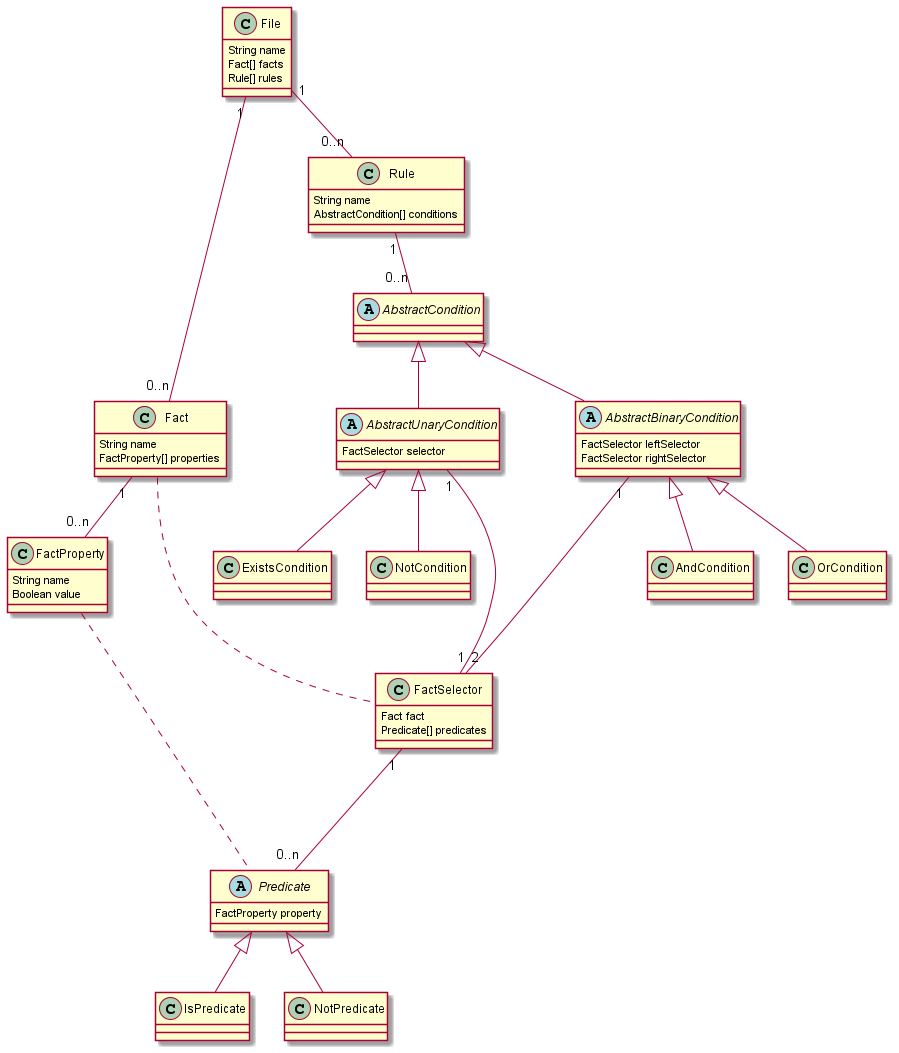
\includegraphics[width=0.95\textwidth]{Sections/images/ReallySimpleRuleLanguage.png}}
    \caption{RSR Concept Hierarchy}
    \label{fig:RSRDiagram}
\end{figure}

This design was then realised in MPS.
As the aim is to attempt different projections we did not initially optimise for editing.
The structure is as show in figure \ref{fig:RSRStructure} and the editors including those shown in figure \ref{fig:RSREditors}.

\begin{figure}
    \centering
    \begin{minipage}{0.30\textwidth}
        \centering
        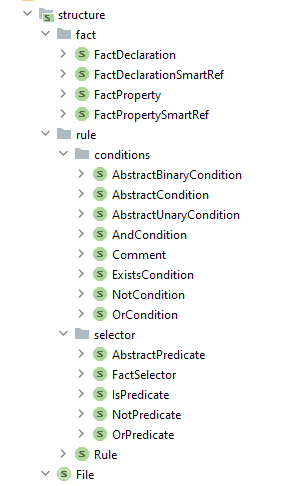
\includegraphics[width=0.9\textwidth]{Sections/images/RSRStructrure.png}
        \caption{RSR}
        \label{fig:RSRStructure}
    \end{minipage}\hfill
    \begin{minipage}{0.70\textwidth}
        \centering
        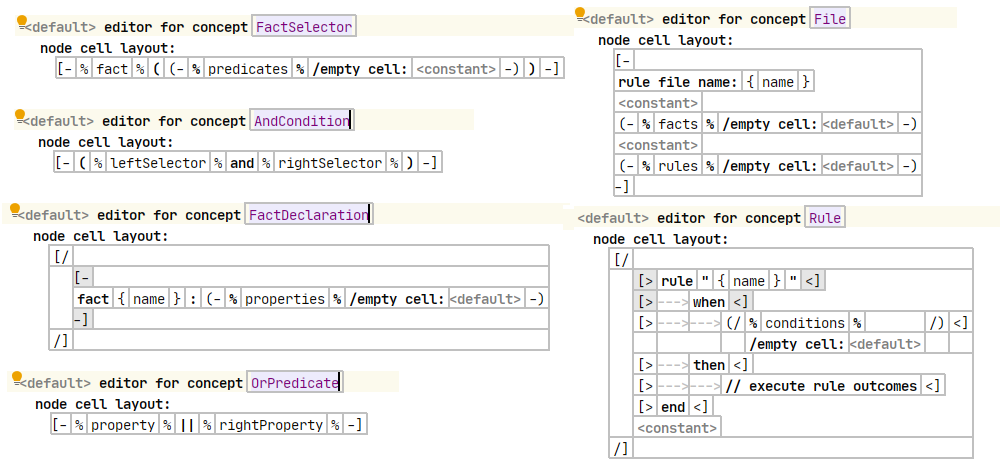
\includegraphics[width=0.9\textwidth]{Sections/images/RSREditors.png} 
        \caption{Editors}
        \label{fig:RSREditors}
    \end{minipage}
\end{figure}

Part of the research question is using projections to reason about large files.
In order to answer this we needed to simulate a large file.
To do this we had to enter a large number of rules.
As this becomes tedious we added a number of editing aids including substitute menus to speed up the entry of conditions, as shown in figure \ref{fig:RSRSubstituteMenu}.
This image, shows that before I had to select an ExistsCondition concept, and thereafter select the Fact for the condition.
After adding the substitute menu, I could immediate select the Fact I wanted and it would then automatically be wrapped with an ExistsCondition node.
I could immediatly select the Fact and the 

\begin{figure}[h]
    \centering
    \fbox{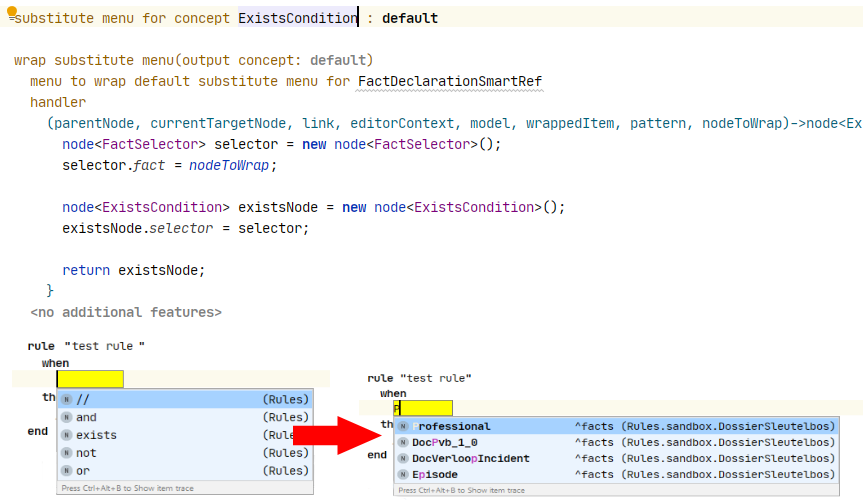
\includegraphics[width=0.95\textwidth]{Sections/images/RSRSubstituteMenu.png}}
    \caption{RSR Substitute Menu}
    \label{fig:RSRSubstituteMenu}
\end{figure}

We also added some intentions to invert incorrectly added conditions.

Finally, we added a constraint to scope the fact properties in predicates to the Fact chosen in the FactSelector.
This made it much easier to select properties in the predicates as indicated in figure \ref{fig:RSRConstraint}.
In the figure you can see that before the scoping constraint it showed a list with dozens of potential FactProperties, that represented all the FactProperties in the Model.
After the constraint is added it only shows the two properties associates with the Fact from the FactSelector.

\begin{figure}[h]
    \centering
    \fbox{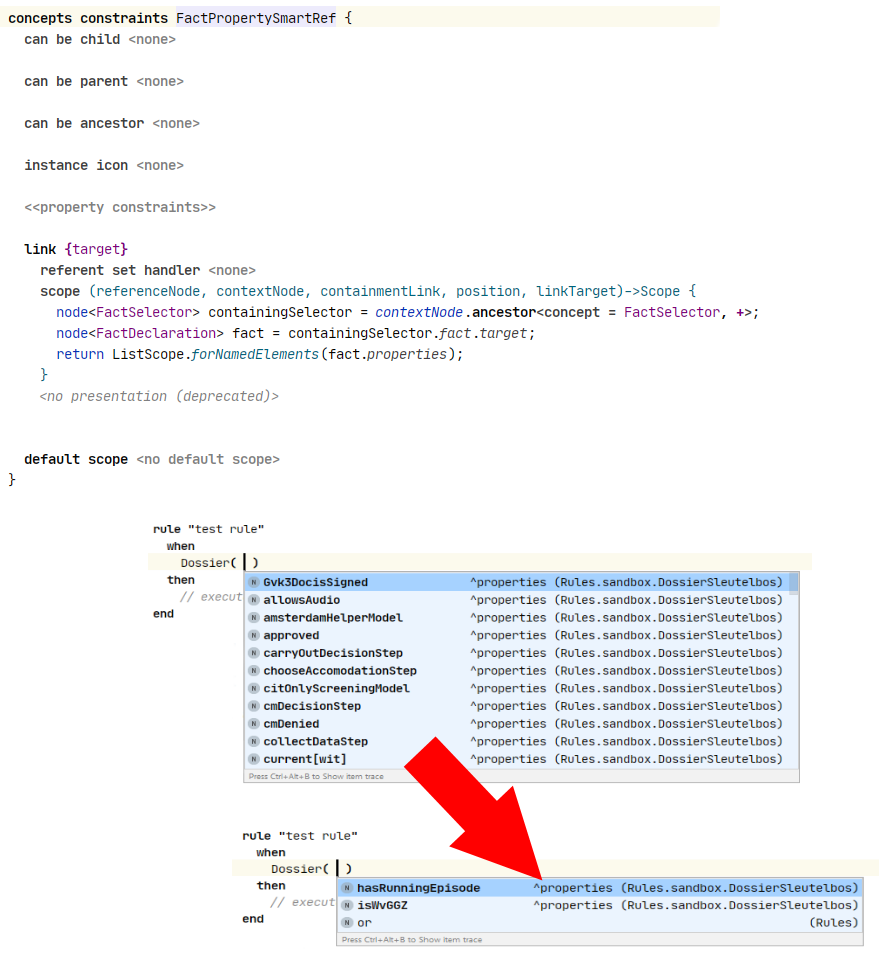
\includegraphics[width=0.95\textwidth]{Sections/images/RSRConstraint.png}}
    \caption{RSR Scoping Constraint}
    \label{fig:RSRConstraint}
\end{figure}

Thus, we have described the entire implementation of the Really Simple Rules Language.

After implementing the language we wrote a program with a large number of rules.
This program on which we will experiment with the different projections.
An example of our default Drools like text projection is show in figure \ref{fig:RSRProgram}.

\begin{figure}[h]
    \centering
    \fbox{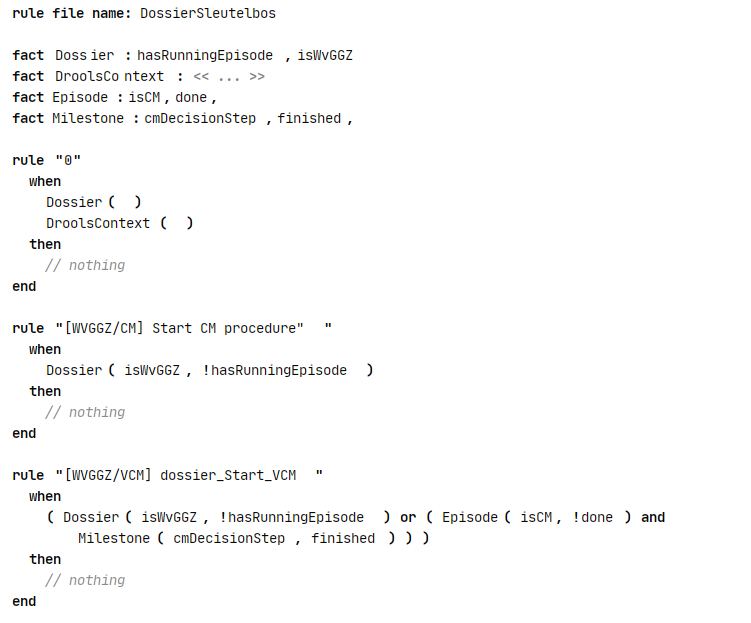
\includegraphics[width=0.95\textwidth]{Sections/images/RSRProgram.png}}
    \caption{RSR program}
    \label{fig:RSRProgram}
\end{figure}

The alternative projections will be discussed in the results section \ref{section:Results_ADR}.

\subsection{Drools-Lite Language}\label{section:DroolsLite}

The RSR was useful as an initial language, however is suffered two major Issues.
Firstly, it's limitations as a language were so great that it was not able to handle many necessary scenarios.
Secondly, our projections would have to be validated by developers with Drools experience.
For this reason we needed to create a projectional language that was much closer to the Drools language.

Our next Language, Drools-Lite, contains many more of the features of Drools.
Our method of selecting the features was to implement the examples that are delivered with Drools (including the corrupt politician example shown in section \ref{section:WhatIsDrools}).
We would implement just enough features to complete the examples.
Whenever we had any queries about how to design the concepts we referred to our analysis of the Drools Language, shown in appendix \ref{appendix:DroolsConceptHierarchy}.
The preliminary design we achieved using this method is shown in figure \ref{fig:DroolsLiteDiagram}.
Later, there were a number of places we diverged a little or merged or decoupled concepts where we thought it would simplify the code.

\begin{figure}[htbp]
    \centering
    \fbox{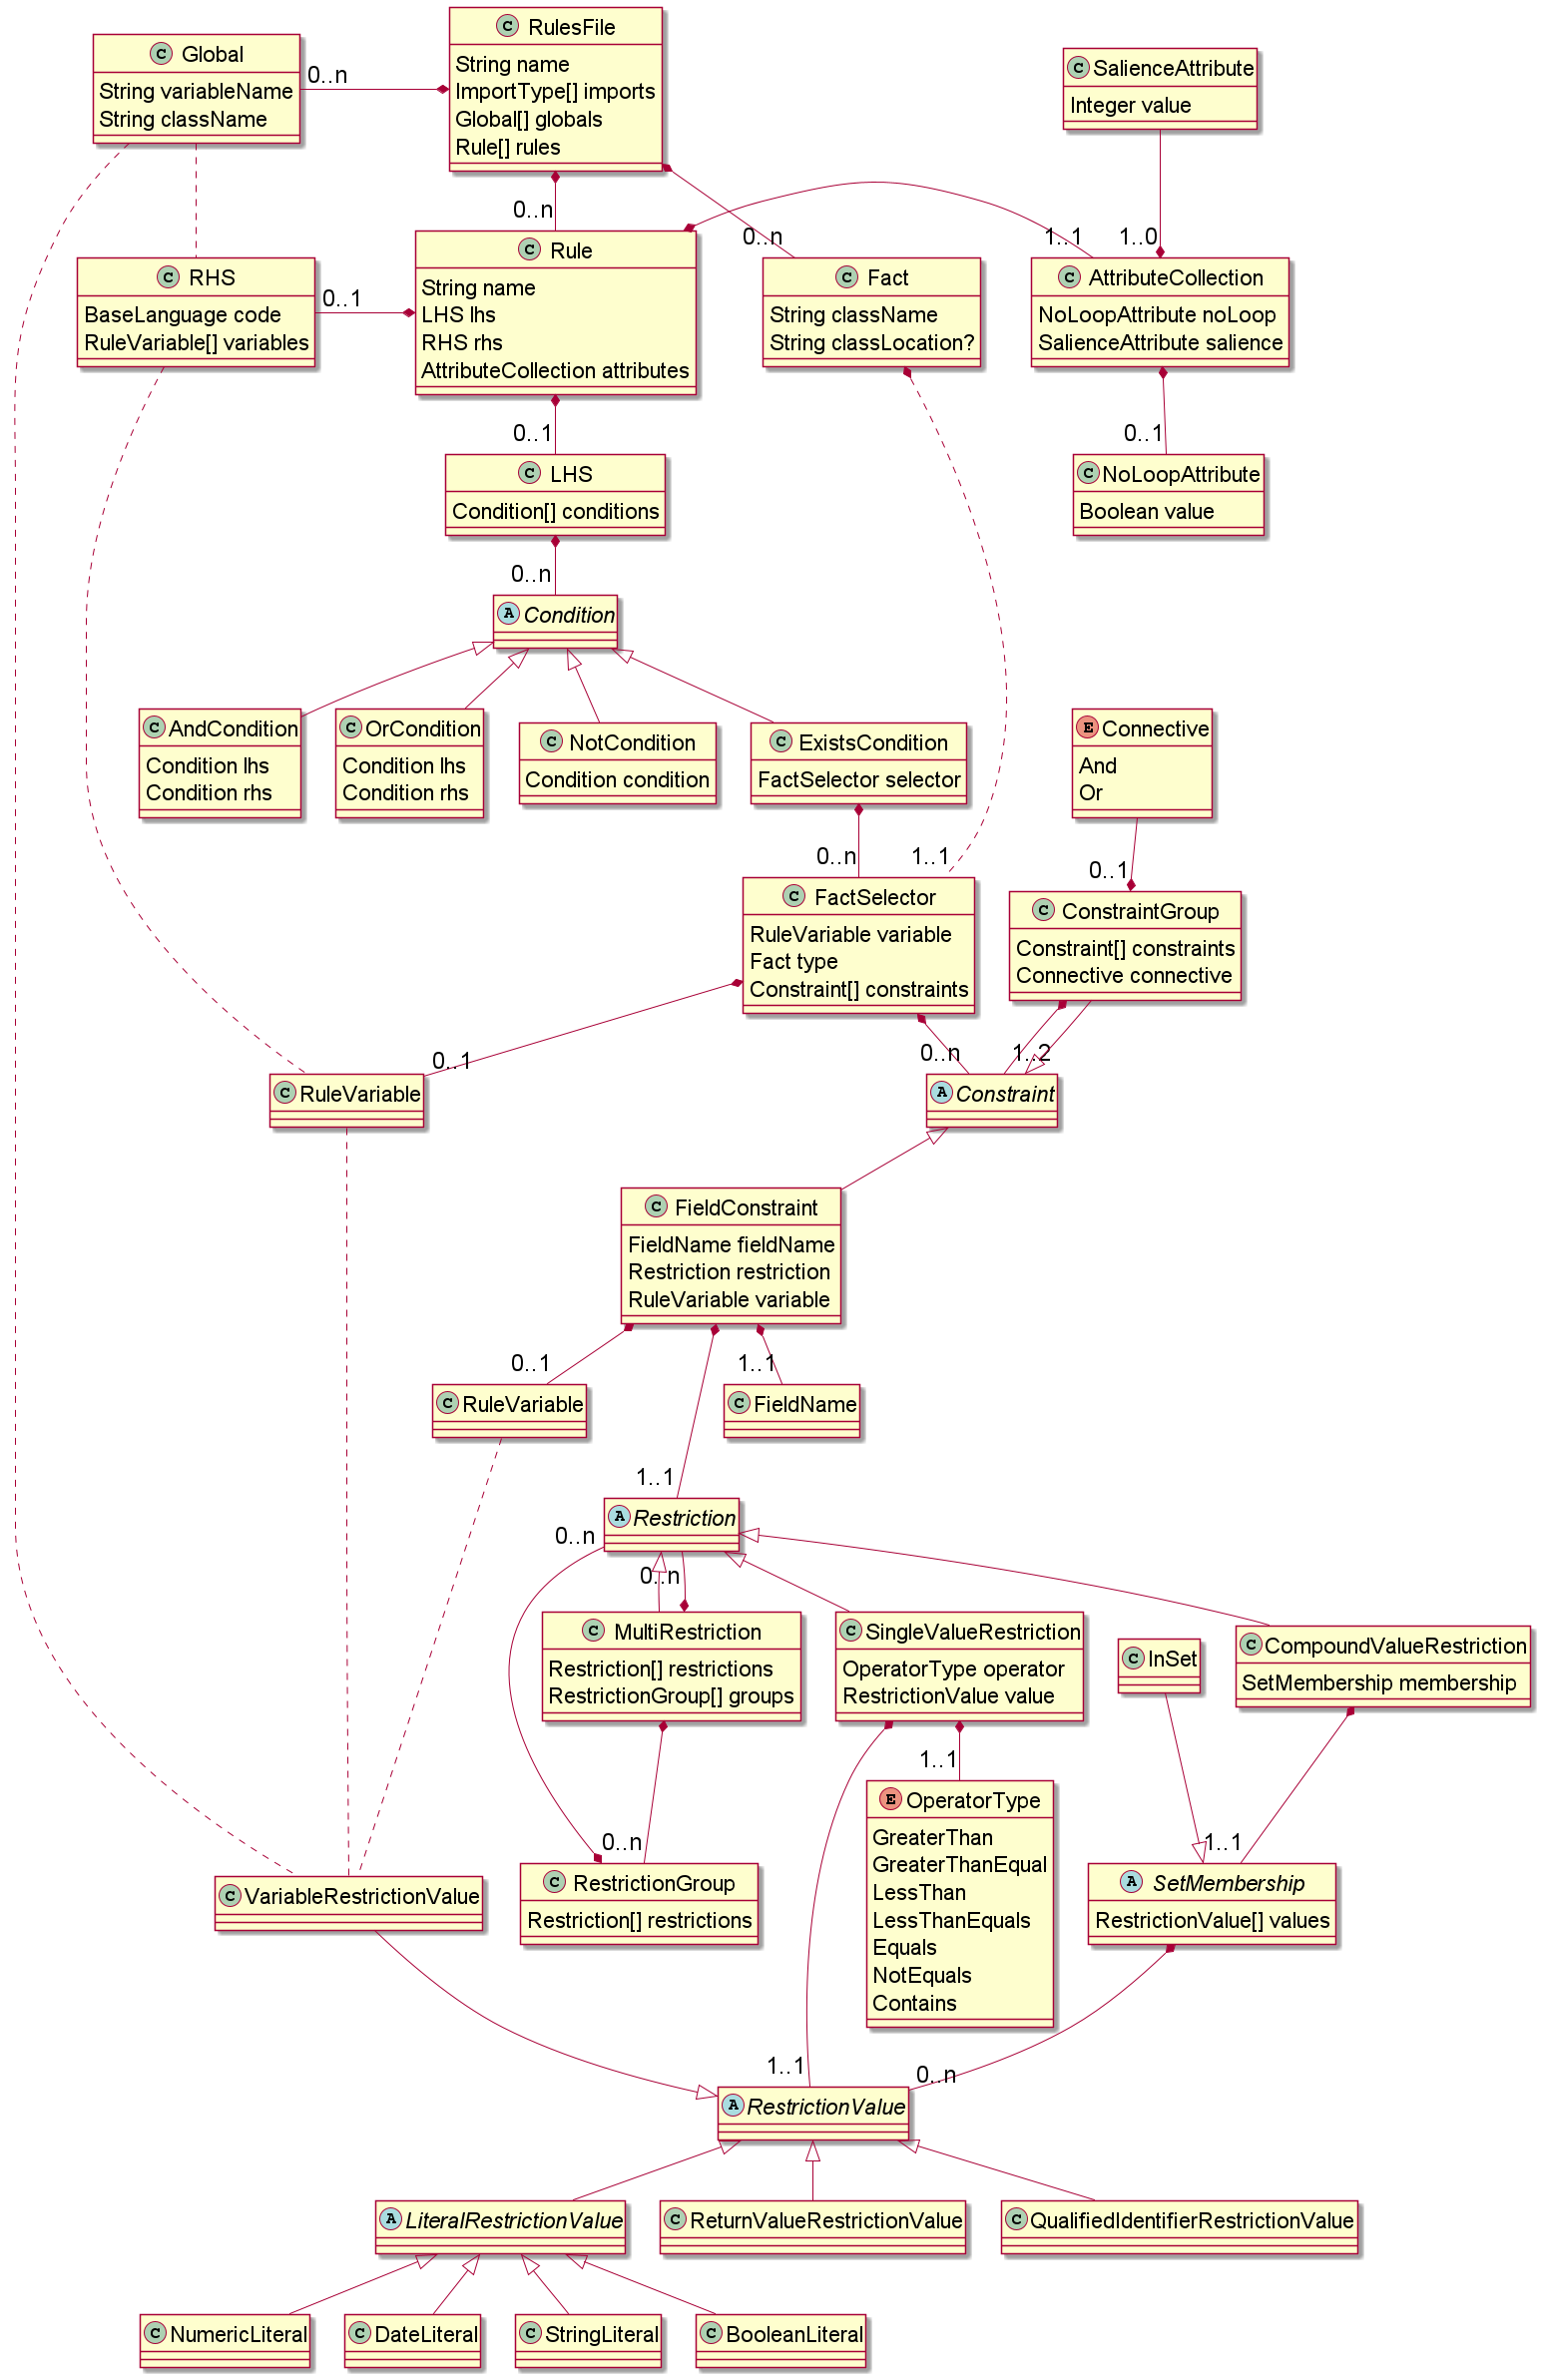
\includegraphics[width=0.85\textwidth]{Sections/images/DroolsLiteStructure.png}}
    \caption{Drools Lite Structure}
    \label{fig:DroolsLiteDiagram}
\end{figure}
 
\paragraph{Rule File} the rule file level statements contains Facts, Globals and Rules.
It also contains semantically unimportant empty lines.

\paragraph{Fact} a fact has a type property.
The type property is implemented using a ClassifierType from the MPS BaseLanguage.
This allows the file to refer to BaseLanguage classes implemented in the same solution or to java JAR files.
We created a smart reference object for this, to take advantage of built in MPS UI functionality.
A smart reference is a node with a single reference of 1:1 cardinality.
The editor builders know how to select which nodes in scope to display to the developer if one uses this object rather than directly referencing the node to which it refers.

In the default editor we use a Read Only Model Access Cell to allow the user to select the type by it's name.
However, once selected it displays the fully qualified name.

\paragraph{FactProperty} In RSR we had FactProperties as children of Facts.
Now that our Facts refer to actual classes, via the Classifier Type, now our FactProperties have to reflect this.
To do this, the Concept itself only has a reference to an InstanceMethodDeclaration, MPS BaseLanguage's definition of a Method signature.
We scoped the concept to only show properties associated with a selected Fact.
Drools interacts with Java objects as if they are Java Beans.
To simulate this we limited the scope of the properties to just getters, i.e. methods that start with "get" or "is" and used a behavior to make sure they displayed without the "get" or "is" prefix.
We also made a smart reference for this concept.

Another option for achieving this is that we could have just wrapped the ClassifierType and referenced its related InstanceMethodDeclarations.
We would have then had to limit the functionality of these items from the BaseLanguage.
Whilst this allows the functionality we wished for, we feel our construction is a little more decoupled that we think properly reflects the structure of the language.
Perhaps if we were to redo this we would have taken the other approach.

\paragraph{Global} Our globals are very simple they have a name and they have a Type, taken from the Base Language.
We have a smart reference, so that it can be used in rules.
The reference extended Expression from the BaseLanguage.
This is, so that we could use it in the Right hand side of the rules.

\paragraph{Rule} Our rules are made of three children, an Attribute collection, A Right hand side and a list of Conditions that make up the left hand side.
We created a component to describe the rule editor, for reuse, as we imagined that we would wrap this in later projections.

\paragraph{Rule Variables} although rule variables do not get created until a FactSelector or a FieldConstrain is used, it is worth mentioning them here, as implicitly they belong to a rule.
A Rule variable only has a name and a type.
We also create a smart reference for it, so it can be used elsewhere within the rule.
Like the global, it extends Expression, to be useable in the Java code of the right hand side.

\paragraph{Right Hand Side}
The right hand side of the rule is for the most part is Java Code.
To implement this, we made the right hand side of the rule a single StatementList.
A StatementList, from the BaseLanguage, as a list of Statements, also from the BaseLanguage, that keeps track of, amongst other things, scope.

There are a number of non-java, Drools specific items that have to go in the right hand side.
Items that had to useable within the righthand side were global variables, rule variables and Drools specific functions.
These all extend Expression, so that they can be seamlessly used.

The Drools specific Methods that are required are Insert, InsertLogical, Modify, Delete and Halt.

\begin{figure}[!h]
    \centering
    \fbox{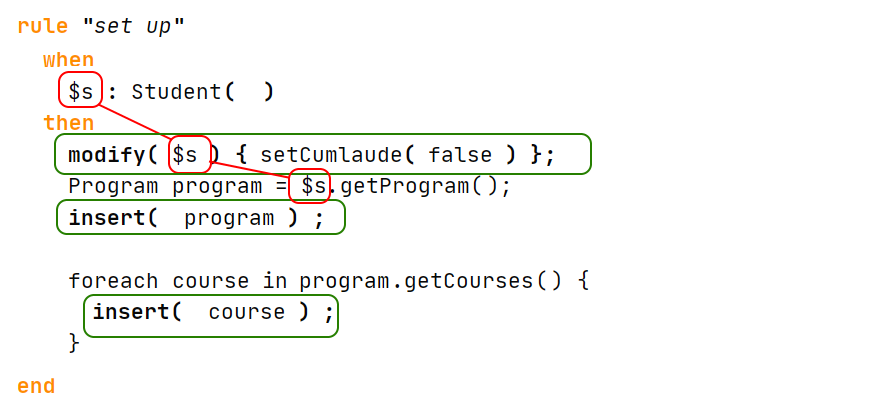
\includegraphics[width=0.70\textwidth]{Sections/images/RHS.png}}
    \caption{RHS}
    \label{fig:RHS}
\end{figure}

Figure \ref{fig:RHS} shows some of the features discussed for the right hand side as shown in our default projection.
The right hand side is represented by the text shown between the \texttt{then} keyword and the \texttt{end} keyword.
In the figure one can see examples of plain Java code, such as assigning to the variable \texttt{program} and the \texttt{foreach} loop.
We can also see that Drools-Lite rule variable \texttt{\$s} is inserted into the Java statements.
We have also highlighted the drools specific methods placed in the code, in this case \texttt{\textbf{modify}} and \texttt{\textbf{insert}}   

\paragraph{RuleAttributes} Rule Attributes is a container to hold all of the attributes that are applicable to a rule.
Initially, we have only implemented the No-Loop and Salience attributes.
These Attributes can only be activated through two intentions we added to the Rule Concept.
We can see, on line 2 in figure \ref{fig:Rule}, an example of the salience attribute added to a rule on line 2.

\emph{Some things to note about figure \ref{fig:Rule}.
We added line numbers to this figure to make it easier to talk about.
The keywords \texttt{rule} on line 1, \texttt{when} on line 3, \texttt{then} on line 6, and \texttt{end} on line 8 have no meaning in the abstract syntax.
They are added to give the developer the same look and feel as a standard Drools file.}

\begin{figure}[h]
    \centering
    \fbox{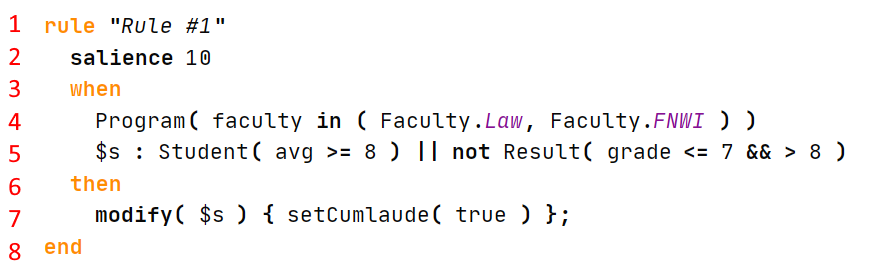
\includegraphics[width=0.85\textwidth]{Sections/images/Rule.png}}
    \caption{Rule}
    \label{fig:Rule}
\end{figure}

\paragraph{Left Hand Side} This is a collection of conditions.
There are four types of conditions.
And, Or, Not and Exists.
And, OR, and Not have one or two children who are also conditions.
Exists contains a FactSelector.

We added dynamic braces, to only show braces around a condition if it is a child of another condition.
This adds visual clarity, without adding unnecessary clutter.
we also added some intentions to make it easy to switch between Exists and Not conditions.

On line 4 in figure \ref{fig:Rule}, the whole line represents an Exists Condition.
Line 5 shows an OR condition with containing an Exists and a Not Condition.
The default editor, through an intention, can make the Exists condition explicit with an \texttt{exists} keyword.
However, the standard practice with Drools developers is to make this implicit, so this is how we show it here.

\paragraph{FactSelector} This always has a reference to a fact.
These facts are \texttt{Program} in line 4 of figure \ref{fig:Rule}, and \texttt{Student} and \texttt{Result} from line 5.

Optionally, the fact selector can be bound to a variable.
In figure \ref{fig:Rule} line 5 the FactSelector referencing the \texttt{Student} Fact is bound to the \texttt{\$s} variable.

The FactSelector also contains a list of constraints on FactProperties, that all must return true in order for the FactSelector to return true.

\paragraph{Constraints} We have three types of constraints.
And and Or constraints contain other constraints.
The FieldConstraints places restrictions on FactProperties.

\paragraph{FieldConstraints}
A FieldConstraint refers to a FactProperty and can be bound to a variable.
It also has a restriction applied to that FactProperty.
Using a substitute menu we wrapped the FactProperty smart reference.
This automatically creates the FieldConstraint from a FactProperty selection by the developer.

There are several types of Restriction and several types of values that they can restrict.

\paragraph{Restriction Values} restriction values that a property can be compared with are as follows.
Literal Restrictions: These are Integer, Float, String, DateTime and Boolean.
Variable Restrictions: these can be global variables, rule variables referring to facts, from the FactSelector, or variables from other FieldConstraints.
Return Value: this is for comparing to anything that can be expressed as an expression, which includes referring to Constants or values behind qualified identifiers.

In figure \ref{fig:Rule} on line 4 we have the return values \texttt{Faculty.Law} and \texttt{Faculty.FNWI}.
on line 5 the literal values \texttt{7} and \texttt{8}.

\paragraph{Restrictions}
A SingleValueRestriction compares a FactProperty against a value.
A MultiRestriction compares a FactProperty against multiple values, not necessarily using the same comparison for each value.
A SetMembership restriction checks if a FactProperty is a member of a group.

In figure \ref{fig:Rule} on line 4 a SetMembership restriction is shown with the \texttt{in ( Faculty.Law, Faculty.FNWI )} text.
Line 5 in the first FactSelector there is the SingleValue restriction \texttt{ avg >= 8}.
The second FactSelector shows a MultiRestrictions \texttt{grade <= 7 \&\& > 8}.

Thus, we have described the pertinent implementation details of the Drools-Lite language.

\subsection{Wireframes}

There are some potential projections we have conceived for which there is not sufficent time to implement.
We would like for these to be assessed and thus would like them to appear as real as possible to the assessors.

Our solution to this conundrum, is to develop these presentations in a wireframing tool.
The Wireframe tool we choose was Axure\cite{Axure_ProductPage}.
We chose thus as we had previous experience of the product.
Also, it is available to students for free.

After much discussion, we settled on two possible projectional programming aids: Truth table and circuit diagram.
We will discuss these in more details in the results section.
